\chapter{Lecture 3: ....}\label{lec:3}
\begin{figure}[H]
    \centering
    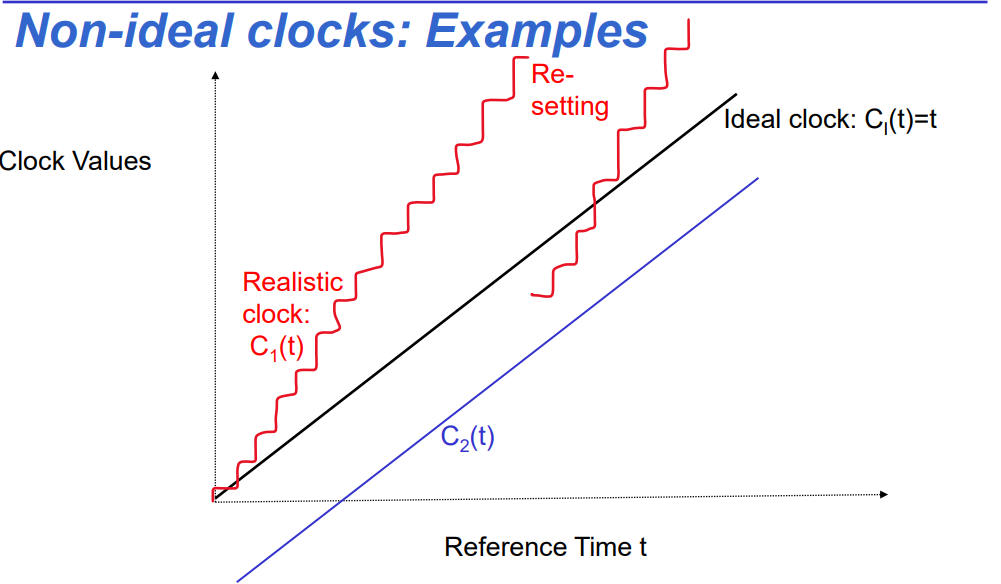
\includegraphics[width=0.9\linewidth]{figures/Lecture3/nonidealclock.png}
    \label{fig:placeholder}
\end{figure}

\section{Time and Clocks in Distributed Systems}

A distributed system consists of \(N\) nodes, where each node has its own
local clock.

The local clock at node \(k\) is denoted by:

\[
C_k(t)
\]

where:

\begin{itemize}
    \item \(t\) = absolute/reference time
    \item \(C_k(t)\) = local clock reading at node \(k\)
\end{itemize}
\begin{table}[h]
\centering
\begin{tabular}{|c|c|c|}
\hline
\textbf{Real time $(t)$} & \textbf{Clock A} & \textbf{Clock B} \\
\hline
10:00:00 & 10:00:01 & 09:59:59 \\
\hline
\end{tabular}
\caption{Example of clock differences in a distributed system}
\end{table}

\subsection{Clock Properties}

\subsubsection{Monotonicity}

A clock should never move backwards:

\[
t_2 > t_1
\quad \Rightarrow \quad
C_k(t_2) \ge C_k(t_1)
\]

This guarantees increasing timestamps.

\subsubsection{Granularity}

Real clocks are discrete rather than continuous.

If a clock updates every \(g\) seconds, then \(g\) is called the
\textbf{granularity}.

Example:

\[
g = 1\text{ ms}
\]
\begin{itemize}
    \item a millisecond clock changes every 1 ms
    \item a microsecond clock changes every 1 μs
\end{itemize}

\subsubsection{Continuous Approximation}

For mathematical analysis, clocks are often modeled as continuous
differentiable functions:

\[
C_k(t)
\]

This allows the use of derivatives to describe clock speed.

\subsection{Clock Drift}

Different clocks run at slightly different rates.

The drift bound is defined as:

\[
\left|
\frac{dC_k(t)}{dt} - 1
\right|
<
\rho_k
\]

where:

\begin{itemize}
    \item \(\frac{dC_k(t)}{dt}\) = rate of the local clock
    \item \(1\) = ideal clock speed
    \item \(\rho_k\) = maximum drift rate
\end{itemize}

Equivalently:

\[
1 - \rho_k
<
\frac{dC_k(t)}{dt}
<
1 + \rho_k
\]

Thus, the clock may run slightly faster or slower than real time.

\subsection{Precision and Accuracy}

\subsubsection{Precision}

Precision measures how closely clocks agree with each other:

\[
|C_i(t)-C_k(t)| \le \pi
\]

where:

\begin{itemize}
    \item \(\pi\) = maximum difference between any two clocks
\end{itemize}

Small \(\pi\) implies tightly synchronized clocks.

\subsubsection{Accuracy}

Accuracy measures how close a clock is to the real/reference time:

\[
|C_i(t)-t| \le \alpha
\]

where:

\begin{itemize}
    \item \(t\) = true UTC/reference time
    \item \(\alpha\) = maximum deviation from real time
\end{itemize}

\subsection{Clock Synchronization}

Because clocks drift over time, distributed systems use synchronization
protocols such as:

\begin{itemize}
    \item NTP (Network Time Protocol)
    \item PTP (Precision Time Protocol)
    \item GPS synchronization
\end{itemize}

The goal is to maintain bounded precision and accuracy.

\section{Coordinated Universal Time (UTC)}

UTC is the international standard time based on atomic clocks.

Characteristics:

\begin{itemize}
    \item adjusted occasionally using leap seconds
    \item distributed via:
    \begin{itemize}
        \item radio signals
        \item GPS satellites
    \end{itemize}
\end{itemize}

Typical accuracy:

\[
\begin{aligned}
\text{Radio signals} &:\quad 0.1\text{ ms} - 10\text{ ms} \\
\text{GPS} &:\quad < 1\mu s
\end{aligned}
\]

\section{Internal Computer Clocks}

Computers maintain hardware counters denoted by:

\[
H_i(t)
\]

The software clock is computed as:

\[
C_i(t)=a_iH_i(t)+b_i
\]

where:

\begin{itemize}
    \item \(a_i\) = scaling factor (clock-rate adjustment)
    \item \(b_i\) = offset correction
\end{itemize}

This allows synchronization software to compensate for clock drift.

\section{Quartz Clock Drift}

Ordinary quartz clocks typically drift by:

\[
\text{approximately 1 second every 11--12 days}
\]

Even small drift accumulates significantly over time.

\section{Applications of Timestamps}

\subsection{Sensor Data}

Timestamps are used for:

\[
\text{measurement ordering}
\]

Applications include:

\begin{itemize}
    \item IoT systems
    \item robotics
    \item distributed sensing
\end{itemize}

\subsection{Event Ordering}

Distributed systems use timestamps to determine:

\[
\text{causality and ordering of events}
\]

\subsection{Authentication}

Authentication systems often require bounded clock differences.

Example:

\[
\text{Ticket valid during interval } [t_1,t_2]
\]

This helps prevent replay attacks.


\section{Clock Synchronisation in Distributed Systems}

\subsection{Problem Setting}

A distributed system consists of \(N\) nodes, each with a local clock \(C_k(t)\), where \(t\) is the real (reference) time.

The main goal is to minimize clock differences:

\[
|C_i(t) - C_k(t)| \le \pi
\]

where \(\pi\) is the maximum allowed precision error.

We distinguish:

\begin{itemize}
    \item \textbf{Internal synchronization}: clocks agree with each other
    \item \textbf{External synchronization}: clocks agree with UTC
\end{itemize}



\section{1. Basic Client--Server Synchronization}

\subsection{Idea}

A client requests the current time from a server.

\subsection{Protocol}

\begin{enumerate}
    \item Client \(A\) sends request to server \(B\)
    \item Server replies with its timestamp:
    \[
    t_B = C_B(t)
    \]
    \item Client knows delay bounds:
    \[
    min \le d \le max
    \]
    \item Client sets its clock to:
    \[
    t_B + \frac{max - min}{2}
    \]
\end{enumerate}


\subsection{Example}

Assume:

\[
t_B = 10:00:00
\quad,\quad
min = 10ms
\quad,\quad
max = 30ms
\]

Then:

\[
\frac{max - min}{2} = 10ms
\]

So client sets:

\[
C_A \leftarrow 10:00:00.010
\]


\subsection{Advantages}

\begin{itemize}
    \item Very simple
    \item Low communication cost
\end{itemize}

\subsection{Disadvantages}

\begin{itemize}
    \item Requires known delay bounds
    \item Sensitive to network jitter
    \item Assumes symmetric delays
\end{itemize}


\section{2. Christian's Method}

\subsection{Idea}

Use measured round-trip time (RTT).

\subsection{Protocol}

\begin{enumerate}
    \item Client sends request
    \item Server replies with timestamp:
    \[
    t_B = C_B(t)
    \]
    \item Client measures RTT:
    \[
    \hat{R}
    \]
    \item Client sets clock:
    \[
    C_A \leftarrow t_B + \frac{\hat{R}}{2}
    \]
\end{enumerate}

\subsection{Example}

Let:

\[
t_B = 10:00:00
\quad,\quad
\hat{R} = 40ms
\]

Then:

\[
\frac{\hat{R}}{2} = 20ms
\]

So:

\[
C_A \leftarrow 10:00:00.020
\]

\subsection{Precision}

\[
\text{Error} \approx \frac{\hat{R}}{2}
\]

\subsection{Advantages}

\begin{itemize}
    \item Works without known delay bounds
    \item Better suited for real networks
\end{itemize}

\subsection{Disadvantages}

\begin{itemize}
    \item Asymmetric delays cause errors
    \item Processing delays distort RTT
    \item Jitter reduces accuracy
\end{itemize}


\section{3. Berkeley Algorithm}

\subsection{Idea}

Internal synchronization using a master node.

\subsection{Protocol}

\begin{enumerate}
    \item Master polls all slaves
    \item Collects clock values
    \item Estimates RTTs
    \item Removes outliers
    \item Computes average time
    \item Sends adjustments to slaves
\end{enumerate}



\subsection{Example}

Assume clocks:

\[
\begin{aligned}
C_1 &= 10:00:05 \\
C_2 &= 10:00:00 \\
C_3 &= 09:59:58 \\
C_4 &= 10:05:00 \; (\text{outlier})
\end{aligned}
\]

Master removes \(C_4\), then computes:

\[
\text{average} \approx 10:00:01
\]

Adjustments are sent:

\[
\Delta_i = \text{avg} - C_i
\]



\subsection{Advantages}

\begin{itemize}
    \item Good internal agreement
    \item Handles faulty clocks (outliers)
    \item No external time source needed
\end{itemize}

\subsection{Disadvantages}

\begin{itemize}
    \item Master is single point of failure
    \item Not UTC accurate
\end{itemize}



\section{4. NTP (Network Time Protocol)}

\subsection{Idea}

Synchronize clocks across the Internet to UTC.

\section{NTP: Hierarchical Organisation (Strata)}
\begin{figure}[H]
    \centering
    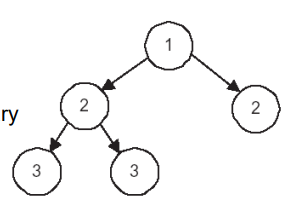
\includegraphics[width=0.5\linewidth]{figures/Lecture3/stratum.png}
    \label{fig:placeholder}
\end{figure}
\subsection{1. What "hierarchy (strata)" means}

In NTP, time servers are organized into levels called \textbf{strata}.

The basic idea is:

\[
\text{closer to the true time source} \;\Rightarrow\; \text{higher quality time}
\]



\subsubsection{Stratum 0}

These are ideal reference time sources (not network machines):

\begin{itemize}
    \item Atomic clocks
    \item GPS satellites
\end{itemize}

They do \textbf{not} send network packets directly.



\subsubsection{Stratum 1}

These are servers directly connected to Stratum 0 sources:

\begin{itemize}
    \item GPS receiver servers
    \item atomic-clock connected servers
\end{itemize}

They represent the \textbf{best available network time servers}.



\subsubsection{Stratum 2}

These servers synchronize from Stratum 1 servers.



\subsubsection{Stratum 3, 4, \dots}

Each level synchronizes from the level above it.



\subsection{2. Why hierarchy is needed}

If all machines synchronized directly to atomic clocks:

\begin{itemize}
    \item overload of Stratum 1 servers
    \item scalability problems
    \item instability under heavy load
\end{itemize}

Instead:

\begin{itemize}
    \item only a few Stratum 1 servers connect to UTC sources
    \item lower strata distribute time further
\end{itemize}



\subsection{3. How synchronization works}
\begin{mdframed}[backgroundcolor=lightgray, linewidth=0pt, innertopmargin=8pt,
innerbottommargin=8pt]
\textbf{Synchronisation Modes}
\begin{itemize}
    \item Multicast (within LAN, using delay assumptions)
    \begin{itemize}
        \item One server broadcasts time to everyone.
    \end{itemize}
    \begin{center}
\begin{tabular}{c}
Server \\
$\downarrow \;\;\;\;\downarrow \;\;\;\;\downarrow$ \\
A \;\;\;\;\;\;\;\; B \;\;\;\;\;\;\;\; C
\end{tabular}
\end{center}
    \item  Client-Server 
    \begin{itemize}
        \item see example under
        \item For widely used (NTP Internet))
    \end{itemize}
    \item Symmetric (peer-2-peer) 
    \begin{itemize}
        \item Every node can talk to every other node 
        \item collects multiple estimates
        \item computes a consensus (often weighted average)
    \end{itemize}
\end{itemize}
\end{mdframed}
\subsubsection{Step 1: Client requests time}

Client sends a request to an NTP server.



\subsubsection{Step 2: Timestamp exchange}

We define four timestamps:

\begin{itemize}
    \item \(T_1\): client sends request
    \item \(T_2\): server receives request
    \item \(T_3\): server sends reply
    \item \(T_4\): client receives reply
\end{itemize}



\subsubsection{Step 3: Delay and offset computation}

Round-trip delay:

\[
d = (T_4 - T_1) - (T_3 - T_2)
\]

Clock offset:

\[
\theta =
\frac{(T_2 - T_1) + (T_3 - T_4)}{2}
\]



\subsubsection{Step 4: Clock update}

The client updates its clock as:

\[
C_{\text{client}} \leftarrow C_{\text{client}} + \theta
\]



\subsection{Interpretation}

Instead of directly setting the clock, the system:

\begin{itemize}
    \item estimates the correct time
    \item then applies a correction (\(\theta\))
\end{itemize}

This avoids sudden jumps in time.



\subsection{4. Reconfiguration on failure}

NTP is fault-tolerant and adapts dynamically.



\subsubsection{Case 1: Primary server loses UTC access}

If a Stratum 1 server loses its GPS/atomic clock source:

\begin{itemize}
    \item it is downgraded to Stratum 2
    \item it is no longer considered a primary time source
\end{itemize}



\subsubsection{Case 2: Server failure}

If a server fails:

\begin{itemize}
    \item clients switch to alternative servers
    \item often within the same or nearby stratum
\end{itemize}


\begin{mdframed}[backgroundcolor=lightgray, linewidth=0pt, innertopmargin=8pt,
innerbottommargin=8pt]
\textbf{Key Intervision of NTP}
\begin{itemize}
    \item Time flows downward from accurate sources (Stratum 0)
    \item Each node corrects itself using upstream servers
    \item The system continuously adapts to failures and network changes
    \item Each message contains time-stamps of recent events
    \begin{itemize}
        \item Local time of send \& receive of previous message
        \item Local time of send of current message
    \end{itemize}
    \item \textbf{Accuracy: LAN ~1ms, Internet ~tens of ms}
\end{itemize}
\end{mdframed}


\section{Summary Comparison}

\[
\begin{array}{|c|c|c|c|}
\hline
\textbf{Method} & \textbf{Idea} & \textbf{Advantage} & \textbf{Weakness} \\
\hline
\text{Client--Server} & Delay bounds & Simple & Needs bounds \\
\hline
\text{Christian} & RTT / 2 & Practical & Asymmetry errors \\
\hline
\text{Berkeley} & Average clocks & Internal consistency & Master failure \\
\hline
\text{NTP} & Hierarchical UTC sync & Scalable & Network jitter \\
\hline
\end{array}
\]
\clearpage
\begin{center}
  {\LARGE\bfseries\color{aaublue}
    MM3 --- Networks and Systems}\\[0.4em]
  {\large\color{accentgray}
    Topic Overview: System-of-Systems Use-Case}\\[0.2em]
  {\large\bfseries
    Digital Twin of Electricity Distribution Grids}\\[0.3em]
  {\small\color{accentgray} Slides 14--26 \quad|\quad
    Hans-Peter Schwefel, Aalborg University}
\end{center}
 
\vspace{0.5em}\hrule\vspace{1em}
 
\begin{summarybox}
\textbf{Core Idea in One Sentence:}\\
The grid has many distributed sensors from different manufacturers
with their own clocks --- combining their data meaningfully requires
understanding and correcting for clock offsets, which is the whole
point of MM3.
\end{summarybox}
 
% ---------------------------------------------------------------
\section{The Physical Setup (Slides 14--17)}
 
The electricity distribution network is organised as a strict
hierarchy, flowing from high voltage down to your home:
 
\begin{center}
\begin{tabular}{ccccc}
\toprule
\textbf{High Voltage} & $\rightarrow$ &
\textbf{Primary Substation} & $\rightarrow$ &
\textbf{MV Grid} \\
& & (e.g.\ 32\,MVA) & & (10--30\,kV) \\
\midrule
\textbf{Secondary Substation} & $\rightarrow$ &
\textbf{LV Grid} & $\rightarrow$ &
\textbf{Your House} \\
(e.g.\ 640\,kVA) & & (400\,V) & & \\
\bottomrule
\end{tabular}
\end{center}
 
\vspace{0.5em}
The \textbf{grid operator} (Distribution System Operator, DSO) has
three overarching goals:
 
\begin{enumerate}[leftmargin=2em, itemsep=4pt]
  \item \textbf{Reliability} --- minimise outage durations and
        prevent overloads or faults.
  \item \textbf{Voltage Quality} --- keep voltage within
        $\pm10\%$ (or $\pm6\%$) of nominal at all connection points.
  \item \textbf{Efficiency} --- minimise energy losses in cables
        and transformers, extend component lifetimes, and target
        investments wisely for renewable integration.
\end{enumerate}
 
Achieving all three requires \emph{real-time visibility} across
the entire grid --- hence the need for dense, distributed
measurements.
 
\begin{notebox}
\textbf{Key numbers to remember:}
\begin{itemize}[itemsep=2pt]
  \item MV grid: 50--500 secondary substations per primary.
  \item LV grid: 1--120 customer connections per secondary
        substation.
  \item Europe loses \textbf{on average $>$7\%} of distributed
        energy to technical losses.
\end{itemize}
\end{notebox}
 
% ---------------------------------------------------------------
\clearpage
\section{What Gets Measured and How (Slides 18--23)}
 
Two main classes of sensor feed data into the digital twin.
 
\subsection{Smart Meters (at Customer Premises)}
 
Smart meters measure electrical consumption, voltage levels,
current, power factor, harmonic distortions, and phase angles.
They typically store \textbf{1-second} resolution data internally
but only transmit \textbf{15-minute averages} (or hourly) to the
DSO remotely, via periodic uploads, alarms, or on-demand access.
 
\subsection{Power Analysers / Measurement Devices (at Substations)}
 
These devices measure voltages per phase, currents, power,
power factor, and harmonics at:
\begin{itemize}[itemsep=3pt]
  \item the busbar of the secondary substation,
  \item each LV feeder (power and current),
  \item optionally junction boxes in the feeder.
\end{itemize}
 
Resolution is typically \textbf{5\,s to 15\,min}, read out via
Modbus locally and connected remotely over fibre or 2--5G.
 
\subsection{What the Data Looks Like}
 
The lecture shows two real-world examples:
 
\begin{itemize}[itemsep=4pt]
  \item \textbf{Denmark, 630\,kVA station, early March (little PV):}
        Active power is always positive (net consumption), peaking
        around 200\,kW during the day, with reactive power showing
        inductive violations at high loads.
  \item \textbf{Germany, 400\,kVA station, end of June (with PV):}
        Active power swings to $-400$\,kW during sunny midday hours
        as local solar generation far exceeds local demand ---
        power flows \emph{back} into the MV grid.
\end{itemize}
\begin{figure}[H]
    \centering
    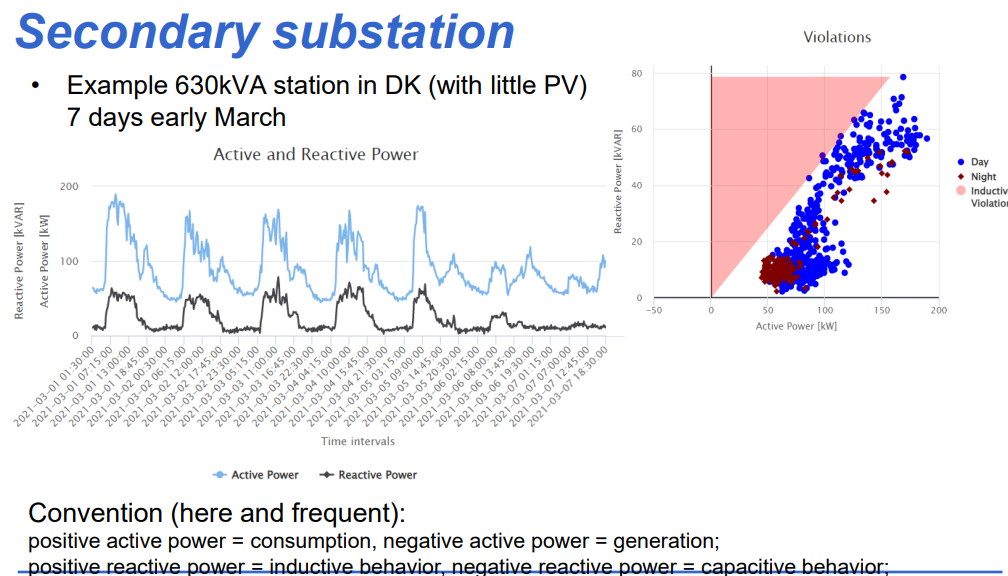
\includegraphics[width=0.9\linewidth]{figures/Lecture3/substationdk.png}
    \label{fig:placeholder}
\end{figure}
\begin{figure}[H]
    \centering
    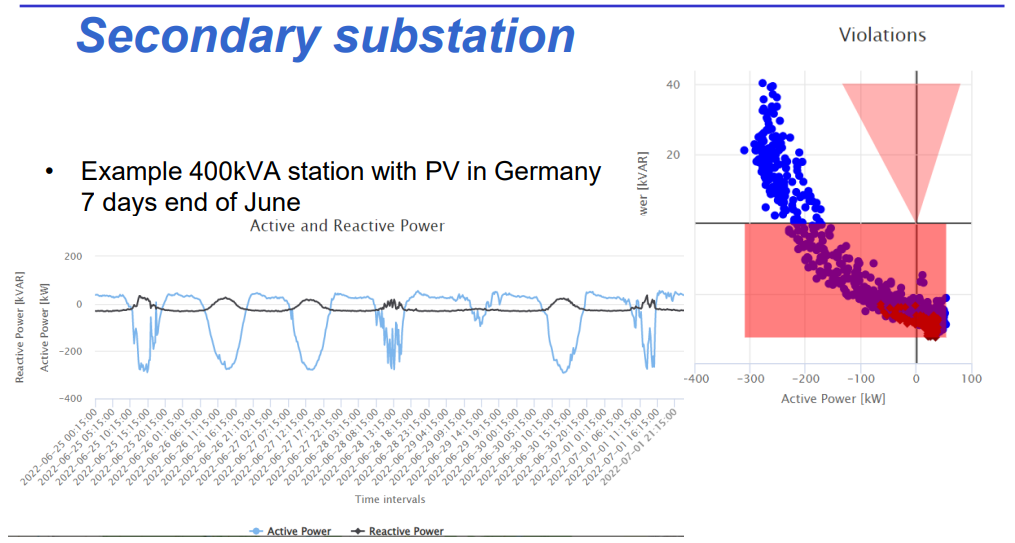
\includegraphics[width=0.9\linewidth]{figures/Lecture3/substationGER.png}
    \label{fig:placeholder}
\end{figure}
 
% ---------------------------------------------------------------
\section{Why This Is Hard --- The Core Problem}
 
\begin{summarybox}
When you combine measurements from different devices (e.g.,
subtracting consumer readings from substation readings to compute
losses), you implicitly assume \textbf{all clocks agree}.\\[4pt]
\textbf{They do not.}
\end{summarybox}
 
Measurement errors come from two sources:
 
\begin{enumerate}[leftmargin=2em, itemsep=4pt]
  \item \textbf{Value errors} --- device class accuracy of
        $0.1\%$--$1\%$, plus transformer errors.
  \item \textbf{Timing errors} --- clock offsets between devices
        cause measurements to cover \emph{different} real-world
        time intervals, even when they are labelled with the same
        timestamp.
\end{enumerate}
 
This motivates the remainder of the lecture: how large are these
timing errors, how do we detect them, and how do we model and
quantify their impact?
 
% ---------------------------------------------------------------
\section{Bridge to the Next Topic}
 
Section~4 of the lecture (slides 32 onwards) takes this problem
further by:
\begin{itemize}[itemsep=3pt]
  \item formally defining the \textbf{time alignment error}
        $\epsilon(T, \delta)$,
  \item modelling consumption measurements as
        \textbf{Markov Modulated Processes} to analytically
        characterise how error grows with clock offset $\delta$,
  \item showing that for a single household with $T=900$\,s,
        the normalised error grows at roughly
        $\alpha \approx 0.4\%$ per second of offset for active
        power, and $\approx 2.6\%$\,/\,s for reactive power.
\end{itemize}
 
\vspace{1em}
\begin{notebox}
\textbf{Practical implication:} A clock offset of just
\textbf{60 seconds} between a smart meter and a substation
analyser can introduce errors of $\sim$24\% in reactive power
loss calculations --- far larger than the device value error
alone.
\end{notebox}

\begin{center}
  {\LARGE\bfseries\color{aaublue}
    MM3 --- Networks and Systems}\\[0.4em]
  {\large\color{accentgray}
    Topic Notes: Impact of Clock Offset on Measurements}\\[0.2em]
  {\large\bfseries Slides 28--45}\\[0.3em]
  {\small\color{accentgray}
    Hans-Peter Schwefel, Aalborg University}
\end{center}
 
\vspace{0.5em}\hrule\vspace{1em}
 
\begin{summarybox}
\textbf{Big picture:} When sensors in a distributed system have
unsynchronised clocks, every averaged measurement covers a
\emph{different} real-world time window. This section quantifies
exactly how large that error is, derives formal metrics, and
builds a stochastic model (Markov Modulated Processes) that lets
us compute error statistics analytically --- without needing the
original high-resolution trace.
\end{summarybox}
 
% ===============================================================
\section{Part I --- Clock Offset and Its Effect on Averaged
Measurements (Slides 28--30)}
 
\subsection{The Measurement Setup}
 
Consider a single sensor measuring a physical quantity $m(t)$
(e.g.\ active power in watts). Rather than reporting every
instantaneous sample, the device reports the \textbf{average}
over a fixed interval of length $T$ (e.g.\ $T = 60$\,s or
$T = 900$\,s):
 
\begin{equation}
  \mhat(T,\,0)
  \;:=\;
  \frac{1}{T}\int_{0}^{T} m(t)\,\mathrm{d}t
  \label{eq:ideal_avg}
\end{equation}
 
This is what an ideal, perfectly synchronised clock would
produce. The interval starts at reference time $0$ and ends at
time $T$.
\begin{figure}[H]
    \centering
    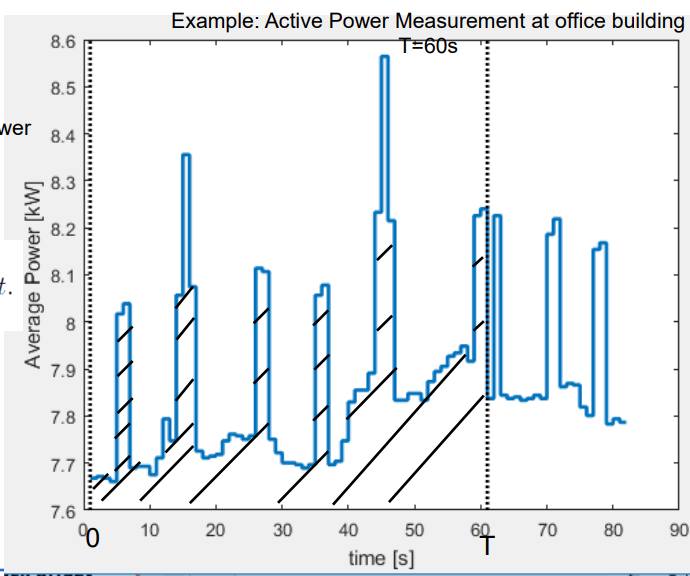
\includegraphics[width=0.7\linewidth]{figures/Lecture3/perfekttimeperiod.png}
    \label{fig:placeholder}
\end{figure}
\subsection{What Happens with a Clock Offset $\delta$?}
 
Suppose the sensor's local clock is ahead (or behind) by
$\delta$ seconds relative to the true reference time. Instead of
integrating over $[0,T]$, the device integrates over
$[\delta,\,T+\delta]$:
 
\begin{equation}
  \mhat(T,\,\delta)
  \;:=\;
  \frac{1}{T}\int_{\delta}^{T+\delta} m(t)\,\mathrm{d}t
  \label{eq:offset_avg}
\end{equation}
 
The two averages $\mhat(T,0)$ and $\mhat(T,\delta)$ cover
overlapping but different windows of the real signal. Visually,
think of sliding the integration window right by $\delta$
seconds: you lose a slice $[0,\delta]$ at the front and gain a
new slice $[T, T+\delta]$ at the back.
\begin{figure}[H]
    \centering
    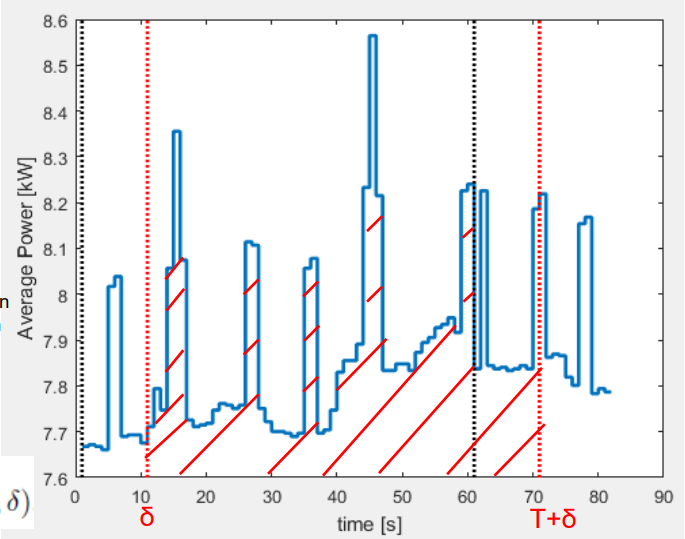
\includegraphics[width=0.7\linewidth]{figures/Lecture3/delayedtimeperiod.png}
    \label{fig:placeholder}
\end{figure}
\begin{notebox}
\textbf{Why does this matter in practice?}
In an electricity distribution grid, the substation meter and
every smart meter at a customer's house each have their own
clock. When you subtract customer readings from the substation
reading to compute energy losses, you are implicitly assuming all
windows are aligned. A clock offset of even a few seconds breaks
this assumption.
\end{notebox}
 
\subsection{The Absolute Measurement Deviation}
 
The \textbf{absolute measurement deviation} caused by a clock
offset $\delta$ is defined as the difference between the ideal
measurement and the offset measurement:
 
\begin{equation}
  \eps(T,\,\delta)
  \;:=\;
  \mhat(T,\,0) \;-\; \mhat(T,\,\delta)
  \label{eq:abs_deviation}
\end{equation}
 
Substituting Equations~\eqref{eq:ideal_avg}
and~\eqref{eq:offset_avg}:
 
\begin{equation}
  \eps(T,\,\delta)
  \;=\;
  \frac{1}{T}\int_{0}^{T} m(t)\,\mathrm{d}t
  \;-\;
  \frac{1}{T}\int_{\delta}^{T+\delta} m(t)\,\mathrm{d}t
  \;=\;
  \frac{1}{T}
  \left[
    \int_{0}^{\delta} m(t)\,\mathrm{d}t
    \;-\;
    \int_{T}^{T+\delta} m(t)\,\mathrm{d}t
  \right]
  \label{eq:dev_expanded}
\end{equation}
 
Equation~\eqref{eq:dev_expanded} makes the intuition precise: the
error is determined entirely by what happens in the two small
\emph{edge slices} of width $\delta$ at the beginning and end of
the interval. If $m(t)$ is roughly constant over these slices,
the error is small. If $m(t)$ changes rapidly (e.g.\ a kettle
switches on), the error can be large.
 
\subsection{Empirical Distribution of the Deviation}
 
The lecture presents an example using 1-second active power
measurements at an office building ($m(t)$ ranges roughly
7600--10\,000\,W with intermittent spikes).
 
For $T = 100$\,s and $\delta = 8$\,s the empirical distribution
of $\eps(T,\delta)$ across all windows in the trace has:
\begin{figure}[H]
    \centering
    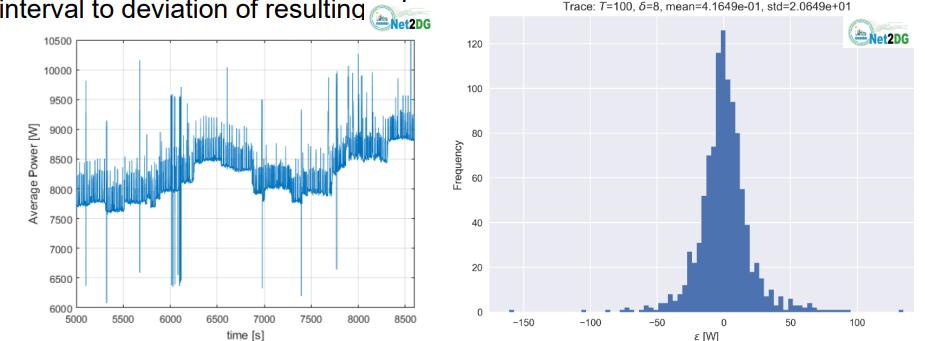
\includegraphics[width=\linewidth]{figures/Lecture3/empiricail.png}
    \label{fig:placeholder}
\end{figure}
\begin{itemize}[itemsep=3pt]
  \item \textbf{Mean} $\approx 0.41$\,W (near zero, as expected
        for a stationary process)
  \item \textbf{Standard deviation} $\approx 20.6$\,W
  \item \textbf{Normalised error} $\approx \mathbf{0.25\%}$ of
        the mean power
\end{itemize}
 
The distribution is roughly bell-shaped and centred near zero,
but has noticeable tails caused by the sharp power transitions
(appliances switching on/off).
 
% ===============================================================
\section{Part II --- Formal Error Metrics (Slide 44)}
 
\subsection{Normalised Time Alignment Error $\kappa$}
 
To compare errors across sensors with different mean power
levels, we normalise the standard deviation of
$\eps(T,\delta)$ by the expected value $\mu$ of the measurand:
 
\begin{equation}
  \kappa(T,\,\delta)
  \;:=\;
  \frac{\mathrm{std}\bigl(\eps(T,\delta)\bigr)}{\mu}
  \label{eq:kappa}
\end{equation}
 
$\kappa$ is dimensionless and expresses the relative spread of
the measurement error as a fraction of the true mean. A value of
$\kappa = 0.01$ means the one-sigma error band is $\pm 1\%$ of
the mean.
 
\subsection{Additive Normalised Time Alignment Error $\alpha$}
 
For small $\delta$, $\kappa(T,\delta)$ grows approximately
linearly in $\delta$. The \textbf{additive normalised time
alignment error} $\alpha$ captures this rate of growth:
 
\begin{equation}
  \alpha(T,\,\delta)
  \;:=\;
  \frac{\mathrm{d}}{\mathrm{d}\delta}\,\kappa(T,\,\delta)
  \;=\;
  \frac{1}{\mu}
  \cdot
  \frac{\mathrm{d}}{\mathrm{d}\delta}\,
  \mathrm{std}\bigl(\eps(T,\delta)\bigr)
  \label{eq:alpha}
\end{equation}
 
The units of $\alpha$ are \emph{percent per second}
(\%\,s$^{-1}$): for every additional second of clock offset,
the normalised error grows by $\alpha$\,\%. This makes $\alpha$
a \textbf{per-device, per-measurand} fingerprint of how sensitive
that sensor's output is to timing errors.
 
\begin{resultbox}
\textbf{Empirical values from ADRES household data
($T = 900$\,s = 15\,min):}
\begin{itemize}[itemsep=3pt]
  \item Single household, \textbf{active power}:
        $\alpha \approx 0.4\%\,\mathrm{s}^{-1}$
  \item Single household, \textbf{reactive power}:
        $\alpha \approx 2.6\%\,\mathrm{s}^{-1}$
\end{itemize}
Reactive power is about $6\times$ more sensitive to clock offsets
than active power, because it fluctuates much more rapidly.
\end{resultbox}
 
\begin{warnbox}
\textbf{Practical implication:} A clock offset of
$\delta = 60$\,s between two devices gives a normalised error
of:
\[
  \kappa \;\approx\; \alpha \times \delta
  \;=\; 2.6\%\,\mathrm{s}^{-1} \times 60\,\mathrm{s}
  \;=\; 156\%
\]
for reactive power --- an error larger than the signal itself.
Even a modest $\delta = 10$\,s gives $26\%$ error. This dwarfs
the $0.1$--$1\%$ value errors of the measurement devices.
\end{warnbox}
 
% ===============================================================
\section{Part III --- Markov Modulated Processes as a Model
for Sensor Data (Slides 31--34)}
 
Rather than always needing the original high-resolution trace to
compute $\kappa$ or $\alpha$, the lecture introduces a stochastic
model that can produce these statistics analytically.
 
\subsection{Continuous-Time Markov Chains: Revision}
 
A \textbf{continuous-time Markov chain (CTMC)} is a stochastic
process $X(t)$ taking values in a finite state space
$E = \{1, 2, \ldots, N\}$ where:
 
\begin{itemize}[itemsep=4pt]
  \item The \emph{future} behaviour depends only on the
        \emph{current} state (Markov property).
  \item Transitions between states are governed by a
        \textbf{generator matrix} (or rate matrix) $Q \in
        \mathbb{R}^{N \times N}$, where:
        \begin{itemize}
          \item $q_{ij} > 0$ for $i \neq j$ is the transition
                rate from state $i$ to state $j$.
          \item $q_{ii} = -\sum_{j \neq i} q_{ij}$, so that
                each row sums to zero:
                $\displaystyle\sum_{j} q_{ij} = 0$.
        \end{itemize}
\end{itemize}
 
For a simple two-state chain the generator looks like:
\[
  Q
  \;=\;
  \begin{pmatrix}
    -q_{12} & q_{12} \\
     q_{21} & -q_{21}
  \end{pmatrix}
\]
 
\subsubsection{State Holding Times}
 
The time spent in state $i$ before jumping to another state is
exponentially distributed with rate $\Lambda_i = -Q_{ii}$:
 
\begin{equation}
  \Pr[D_i \leq t]
  \;=\;
  1 - e^{-\Lambda_i\, t},
  \qquad t \geq 0
  \label{eq:holding}
\end{equation}
 
\subsubsection{State Probability Evolution}
 
Let $\mathbf{P}(t)$ be the row vector of state probabilities at
time $t$. Given initial distribution $\mathbf{P}(0)$:
 
\begin{equation}
  \mathbf{P}(t)
  \;=\;
  \mathbf{P}(0)\,e^{Qt}
  \label{eq:state_prob}
\end{equation}
 
where $e^{Qt}$ is the matrix exponential of $Qt$.
 
\subsubsection{Steady-State Distribution}
 
As $t \to \infty$, the chain converges (for irreducible,
positive-recurrent chains) to a steady-state distribution $\pi$
satisfying:
 
\begin{equation}
  \pi Q = \mathbf{0},
  \qquad
  \pi\,\mathbf{1}^{\top} = 1
  \label{eq:steadystate}
\end{equation}
 
where $\mathbf{1}$ is a column vector of ones.
 
\subsection{Markov Modulated Process (MMP)}
 
A \textbf{Markov Modulated Process} (MMP) extends the CTMC by
attaching a \emph{value} to each state. For power modelling:
 
\begin{itemize}[itemsep=4pt]
  \item The chain $X(t)$ with generator $Q$ describes how the
        power level switches over time.
  \item A diagonal matrix $E$ encodes the power consumed in each ($E_{ii}$ power
consumed while in State i)
        state:
        \[
          E
          \;=\;
          \mathrm{diag}(e_1,\, e_2,\, \ldots,\, e_N)
        \]
        where $e_i$ is the active power (in kW) while the process
        is in state $i$.
\end{itemize}
 
The measurand $m(t)$ at any instant is simply $e_{X(t)}$.
Because $X(t)$ is Markov, the full statistics of the time-averaged
$\mhat(T,\delta)$ and hence of $\eps(T,\delta)$ can be computed
analytically from $Q$ and $E$ --- no simulation of the original
trace is needed.
\begin{figure}[H]
    \centering
    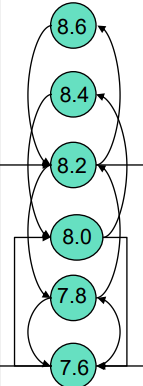
\includegraphics[width=0.2\linewidth,angle=90]{figures/Lecture3/markovmodulated.png}
    \label{fig:placeholder}
\end{figure}
\subsection{Why MMP Fits Power Data}
 
Office and household loads switch between a small number of
identifiable power levels (e.g.\ baseline load $\approx 7.6$\,kW,
medium load $\approx 8.0$\,kW, peak load $\approx 8.6$\,kW for
the office example in the lecture). The inter-event times between
level changes are well approximated by exponential distributions,
making a CTMC a natural fit.
 
\subsection{Fitting the MMP to a Measured Trace}
 
Given a high-resolution trace represented as a sequence of
$(t_i, v_i)$ pairs, where $t_i$ is the time of the $i$-th
transition and $v_i$ is the new value, the fitting procedure is:
 
\begin{enumerate}[leftmargin=2em, itemsep=6pt]
  \item \textbf{Discretise} the observed values $v_i$ into $N$
        representative levels $d_1 < d_2 < \cdots < d_N$
        (e.g.\ equidistant bins spanning the observed range).
 
  \item \textbf{Estimate the embedded transition matrix $P$} of
        the discrete-time chain observed at transition moments:
        \begin{equation}
          p_{ij}
          \;=\;
          \frac{\#\text{transitions from level }i\text{ to level }j}
               {\#\text{transitions away from level }i}
          \label{eq:pij}
        \end{equation}
 
  \item \textbf{Estimate the total leaving rate} for each state
        from the mean holding time in that state:
        \begin{equation}
          \Lambda_i
          \;=\;
          \frac{1}{\overline{D}_i}
          \label{eq:lambda_i}
        \end{equation}
        where $\overline{D}_i$ is the sample mean of all observed
        holding times in state~$i$.
 
  \item \textbf{Construct the generator matrix} by distributing
        the total leaving rate over the outgoing transitions:
        \begin{equation}
          q_{ij}
          \;=\;
          \Lambda_i \cdot p_{ij},
          \qquad i \neq j
          \label{eq:qij}
          \qquad\Longrightarrow\qquad
          Q_{ii} = -\Lambda_i
        \end{equation}
\end{enumerate}
 
\begin{notebox}
\textbf{Interpretation of Equation~\eqref{eq:qij}:}
The rate $q_{ij}$ at which the process jumps from $i$ to $j$ is
the overall rate of leaving $i$ (given by $\Lambda_i$) multiplied
by the probability of going to $j$ specifically (given by
$p_{ij}$). This is the standard relationship between a
continuous-time chain and its embedded discrete-time chain.
\end{notebox}
 
\subsection{The MMP Gap-T Extension}
\todo{need to look further at this dont quite understand yet}
The basic MMP describes the instantaneous power statistics well,
but to compute $\eps(T,\delta)$ we also need to capture
\textbf{temporal correlations} across an interval of length $T$
(which can be 900\,s for 15-minute averages). The
\textbf{MMP Gap-T model} handles this:
 
\begin{enumerate}[leftmargin=2em, itemsep=5pt]
  \item Use $Q$ (and its matrix exponential $e^{Q\delta}$) to
        model the detailed evolution of $m(t)$ within the two
        small edge slices $[0,\delta]$ and $[T, T+\delta]$.
  \item Use the \textbf{transition probability matrix}
        $P_T = e^{QT}$ to describe how the state evolves across
        the large gap $[0,T]$, without tracking every detail in
        between.
\end{enumerate}
 
The autocorrelation comparison in the lecture (slide~43) shows
that the MMP simulation decays to zero much faster than the real
trace, which has long-range correlations over hundreds of
seconds. The MMP Gap-T model corrects this by incorporating
$P_T$ for the correct long-range correlation structure.
\begin{figure}[H]
    \centering
    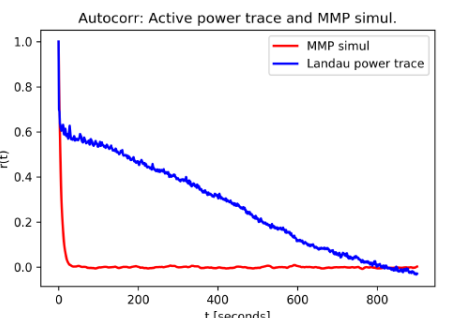
\includegraphics[width=0.6\linewidth]{figures/Lecture3/autocorr.png}
    \label{fig:placeholder}
\end{figure}
% ===============================================================
\section{Behavior of Normalized Time Alignment
Error for increasing clock deviation (STILL NEED TO MAKE)}
\todo{Don't know what this means yet still need to look at}
\begin{figure}[H]
    \centering
    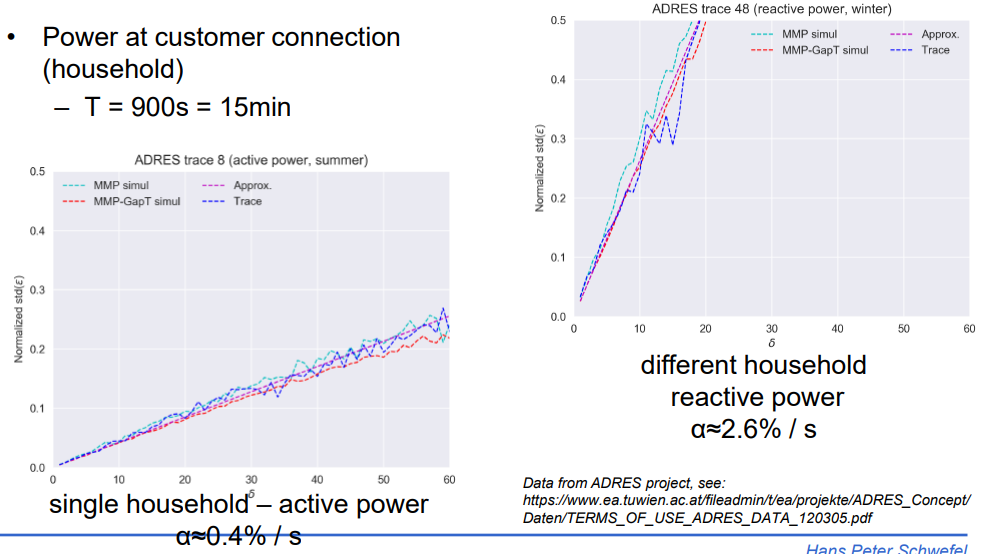
\includegraphics[width=\linewidth]{figures/Lecture3/IDKyet.png}
    \label{fig:placeholder}
\end{figure}
\section{Part IV --- Use-Case: Grid Loss Calculation
(Slides 37--38)}
 
\subsection{Why Losses Require Joint Measurements}
 
Grid energy losses are computed by comparing energy flowing
\emph{into} a section of the network against energy flowing
\emph{out}. This requires measurements at multiple points to be
\textbf{time-aligned}. Two standard approaches:
 
\subsubsection{Method 1: Total Loss from Energy Balance}

The idea is simple in principle: energy flowing \emph{into} a
section of the network minus energy flowing \emph{out} equals
what was lost as heat. In terms of averaged powers over interval
$T$:

\begin{equation}
  L_1
  \;=\;
  T \cdot
  \left(
    P^{(0)}_{\mathrm{imp}} - P^{(0)}_{\mathrm{exp}}
    +
    \sum_{j=1}^{K}
    \Bigl(P^{(j)}_{\mathrm{inj}} - P^{(j)}_{\mathrm{cons}}\Bigr)
  \right)
  \label{eq:L1}
\end{equation}

where $P^{(0)}_{\mathrm{imp}}$ and $P^{(0)}_{\mathrm{exp}}$ are
the import and export powers at the primary substation busbar,
and the sum runs over $K$ customer connections, each contributing
an injected power (e.g.\ from rooftop PV) and a consumed power
measured by a smart meter.

\paragraph{Why clock offsets destroy $L_1$.}
To see the problem concretely, imagine the substation pushes out
206\,kW while customers collectively consume 200\,kW, so the
true cable loss is 6\,kW --- about 3\% of total flow. Now
suppose one smart meter has a clock offset of $\delta = 8$\,s.
During those 8 extra seconds, a washing machine switches on, so
that meter reports 205\,kW instead of 200\,kW for its window.
The computed loss becomes $206 - 205 = 1$\,kW instead of
6\,kW: an 83\% error from a timing slip of 8 seconds.

The offset did not dramatically change any individual large
reading --- 200\,kW became 205\,kW, a shift of only 2.5\%. But
because $L_1$ works by \emph{subtracting} many large numbers to
find a small remainder, even a modest shift in one term
dominates the result. This is the numerical phenomenon of
\textbf{catastrophic cancellation}: when you subtract two large,
nearly equal numbers, the answer is small and the relative
contribution of any error is amplified. Grid losses being only
2--7\% of total power flow means the numbers being subtracted
are almost equal by design, making $L_1$ structurally
vulnerable. The lecture (slide~48) shows this plays out to
errors of \textbf{thousands of percent} for offsets above
30--60 seconds..

\subsubsection{Method 2: Technical Loss from Ohmic Heating}

\begin{equation}
  L_2
  \;=\;
  T \cdot \sum_{j=1}^{C} I_j^2\, R_j
  \label{eq:L2}
\end{equation}

where the sum runs over all $C$ cable segments, with $I_j$ the
RMS current in segment $j$ and $R_j$ its resistance (a fixed,
known physical parameter of the cable).

This formula comes directly from Joule's law: a current $I$
flowing through a resistance $R$ dissipates power $I^2 R$ as
heat. Integrating over time $T$ gives the energy lost.

\paragraph{Why $L_2$ is robust to clock offsets.}
There are two structural reasons:

\begin{enumerate}[leftmargin=2em, itemsep=5pt]
  \item \textbf{No cross-device subtraction.} Each term
        $I_j^2 R_j$ is computed entirely from a single sensor
        on a single cable segment. There is no subtraction of
        one device's reading from another's. Clock offsets on
        different devices therefore cannot interfere with each
        other --- a timing error on sensor $j$ can only affect
        term $j$, and only by a small amount.

  \item \textbf{Current changes slowly and smoothly.}
        Recall from Equation~\eqref{eq:dev_expanded} that the
        deviation $\epsilon(T,\delta)$ depends on what happens
        in the two edge slices of width $\delta$ at the
        boundaries of the integration window. For active power
        at a single household, these slices can be very
        different from the rest of the window because appliances
        switch on and off abruptly. Cable currents, by contrast,
        are aggregates of many customers' loads --- individual
        spikes average out --- so $I_j(t)$ varies slowly and
        the edge-slice values are close to the window average.
        The resulting $\epsilon$ on each $I_j^2 R_j$ term is
        therefore small.
\end{enumerate}

\begin{notebox}
\textbf{The trade-off.} $L_2$ requires a current sensor on
\emph{every} cable segment in the feeder, which may mean
dozens of additional measurement devices per substation. $L_1$
only needs one meter at the substation plus the existing smart
meters at customers --- infrastructure that is often already
deployed. In practice, $L_2$ is more accurate but far more
expensive to instrument.
\end{notebox}
 
\subsection{Key Result from the Loss Calculation Study}
 
The lecture shows a log-scale plot of relative loss deviation as
a function of $\delta$ (for $T = 900$\,s, afternoon trace):
 
\begin{itemize}[itemsep=4pt]
  \item \textbf{Total loss $L_1$} (solid line): error grows
        rapidly from near 0 at $\delta = 0$ and reaches
        \textbf{thousands of percent} for $\delta \sim 120$\,s.
        The loss calculation essentially becomes meaningless for
        offsets above a few tens of seconds.
  \item \textbf{Technical loss $L_2$} (dashed line): error is
        much smaller and saturates around 10\,\% for large
        $\delta$, because $I^2$ changes more smoothly than the
        difference of two power readings.
\end{itemize}
\begin{figure}[H]
    \centering
    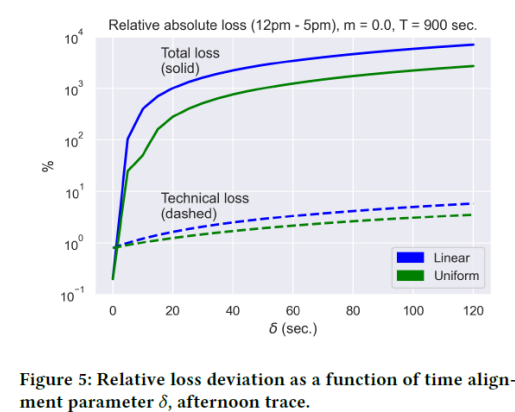
\includegraphics[width=0.7\linewidth]{figures/Lecture3/L1vsL2.png}
    \label{fig:placeholder}
\end{figure}
\begin{warnbox}
\textbf{Bottom line:} The energy-balance method $L_1$ is
\emph{extremely} sensitive to clock offsets. For NTP-synchronised
devices on the Internet (typical offset: tens of milliseconds to
a few seconds), $L_1$ may still be acceptable. But for devices
that have drifted by 30--120 seconds (e.g.\ after a reboot or
GPS loss), the computed losses are completely unreliable.
\end{warnbox}
 
% ===============================================================
\section{Summary of All Key Equations}
 
\begin{center}
\renewcommand{\arraystretch}{2.0}
\begin{tabularx}{\textwidth}{@{} l X @{}}
\toprule
\textbf{Symbol / Equation} & \textbf{Meaning} \\
\midrule
$\displaystyle
  \mhat(T,\delta) = \frac{1}{T}\int_{\delta}^{T+\delta}m(t)\,\mathrm{d}t$
& Averaged measurement over interval $[\delta, T+\delta]$ \\
 
$\displaystyle
  \eps(T,\delta) = \mhat(T,0) - \mhat(T,\delta)$
& Absolute deviation caused by clock offset $\delta$ \\
 
$\displaystyle
  \kappa(T,\delta) = \frac{\mathrm{std}(\eps(T,\delta))}{\mu}$
& Normalised time alignment error (dimensionless, in \%) \\
 
$\displaystyle
  \alpha(T,\delta) = \frac{\mathrm{d}}{\mathrm{d}\delta}\,\kappa(T,\delta)$
& Additive normalised time alignment error (\%/s) \\
 
$\displaystyle
  \Pr[D_i \leq t] = 1 - e^{-\Lambda_i t}$
& Exponential holding time in CTMC state $i$ \\
 
$\displaystyle
  \mathbf{P}(t) = \mathbf{P}(0)\,e^{Qt}$
& State probability evolution via matrix exponential \\
 
$\displaystyle
  \pi Q = \mathbf{0},\quad \pi\mathbf{1}^\top = 1$
& Steady-state equations for CTMC \\
 
$\displaystyle
  q_{ij} = \Lambda_i \cdot p_{ij}$
& Generator rate from embedded chain + holding times \\
 
$\displaystyle
  L_1 = T\!\left(P^{(0)}_{\mathrm{imp}} - P^{(0)}_{\mathrm{exp}}
  + \sum_j(P^{(j)}_{\mathrm{inj}} - P^{(j)}_{\mathrm{cons}})\right)$
& Total loss via energy balance \\
 
$\displaystyle
  L_2 = T\sum_{j=1}^{C} I_j^2 R_j$
& Technical loss via ohmic heating \\
\bottomrule
\end{tabularx}
\end{center}

